\documentclass{article}
\usepackage[includeheadfoot,margin=1.0in]{geometry}
\usepackage{amsfonts}
\usepackage{amsmath}
\usepackage{amssymb}
\usepackage{fancyhdr}
\usepackage{hyperref}
\usepackage{graphicx}
\usepackage{multicol}
\usepackage[dvipsnames]{xcolor}
\begin{document}
%
% Set Title/Author
%
\title{Legend of the Great Unwashed \\ player Manual}
\author{Team USA \\ Software Engineering \\ Sam Houston State University}
%
% Set page styles
%
\pagestyle{fancy}
\fancyhead[LE,RO]{User Manual}
\fancyhead[RE,LO]{\leftmark}
\fancyfoot[RE,LO]{}
\renewcommand{\headrulewidth}{2pt}
\renewcommand{\thefootnote}{[\arabic{footnote}]}
%
% Generate Title
%
\maketitle
\newpage
%
% Generate Table of Contents
%
\tableofcontents
\newpage
%
% Begin
%
\section{About}
	Legend of the Great Unwashed is a point-and-click adventure game that falls within the ``room escape'' genre. As such, the player will be expected to find inconspicuous items to solve puzzles that allow their advancement through the game's various puzzles. 
	
	Legend of the Great Unwashed was created by TeamUSA of Sam Houston State University's Fall 2015 Software Engineering Course. TeamUSA consists of Jordan Sparks, Derek Menteer, John Zhang, Vincent Sanchez, Pramesh Bhandari, and Andrew McGowen. Juan Carmona is a former team member. 
\section{Story}
	The player takes on the role of a student in Dr. Burris's Data Structures and Algorithms class. It is the end of the semester, and a final lab must be turned in to assure a passing grade. Because Dr. Burris has a certain aversion to those who procrastinate, he has laid out a maze of puzzles and traps inside AB1 to prevent those poor souls, the great unwashed, from succeeding in escaping his class with their GPAs intact. 
\section{Gameplay}
	\subsection{Main Menu}
		The main menu allows the player to create a new game, load a previous save, or exit the application.
		\begin{center}
			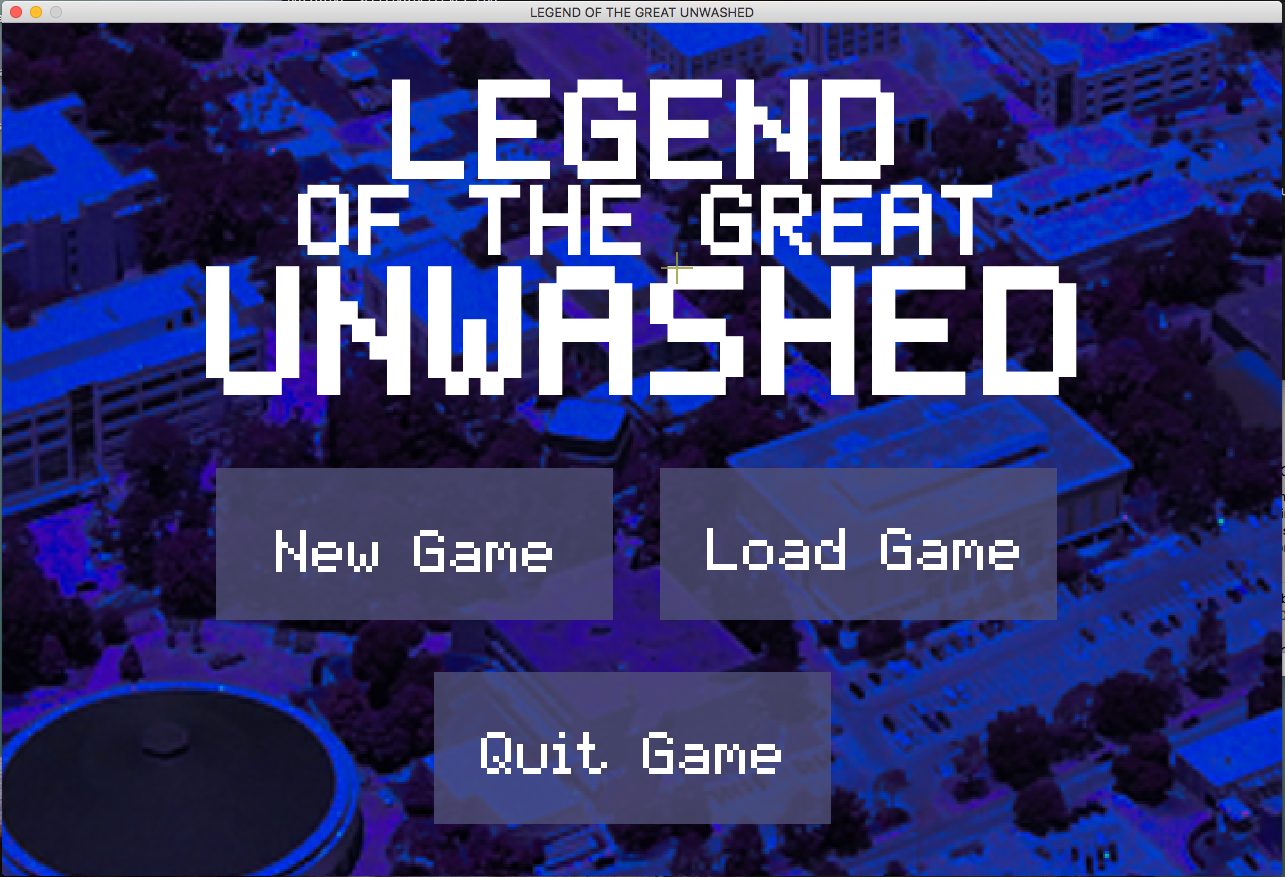
\includegraphics[scale=0.3]{UMimages/mainMenu}
		\end{center} 
	\subsection{Interface}
		The player interacts with the game via a standard two button mouse, and is represented on-screen by a cursor. This cursor can be one of three different types, depending on its position within the game window:
		\begin{itemize}
			\item The default cursor: 
\includegraphics[scale=0.2]{UMimages/Default}
			\item The directional cursor: 
\includegraphics[scale=0.2]{UMimages/Up}
\includegraphics[scale=0.2]{UMimages/Down}
\includegraphics[scale=0.2]{UMimages/Left}
\includegraphics[scale=0.2]{UMimages/Right}
			\item The select cursor: 
\includegraphics[scale=0.04]{UMimages/Select}
		\end{itemize}
		The default cursor is active whenever the player is not within a click region for either movement or an inventory collectible. \footnote{The select cursor \emph{does not} appear when the player hovers over easter eggs!} The movement cursors will appear when the player is within a click region that would transition them to a new scene within the game, but will not appear when the cursor is in a click region that would simply generate a text box. For example, a player in a click region that would turn their perspective to the right would see 
\includegraphics[scale=0.15]{UMimages/Right}, instead of the default cursor. Finally, the select cursor appears when and only when the player is inside the click region for a collectible inventory item.\footnote{Knowing this, the select cursor can be useful for finding hidden inventory items.}
		
		It is also important to note that each scene of gameplay typically will have differing click regions for player movement. While a majority of scenes can be relied on to have a ``go back'' region along the bottom edge of the window, certain scenes within the game do not have this ability, for reasons that will become apparent during the course of gameplay. An example of what to expect for region positioning follows:\footnote{The player will not see the blue click boxes during normal gameplay. These are for demonstration purposes only.}
		\begin{center}
			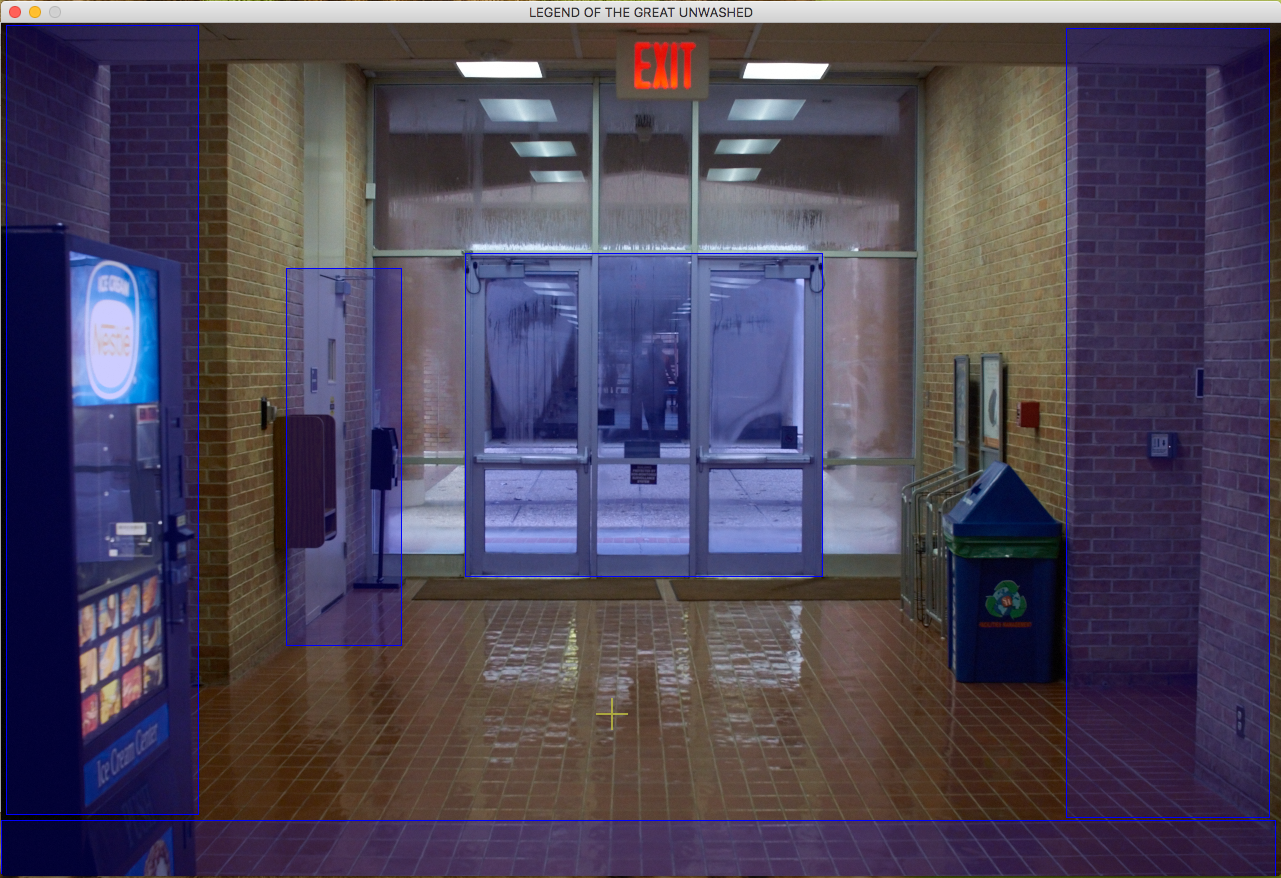
\includegraphics[scale=0.3]{UMimages/clickDemo}
		\end{center}
		Finally, certain regions in the game will generate text boxes, play audio, or cause another event to occur besides moving the player. These regions will show the default cursor (
\includegraphics[scale=0.15]{UMimages/Default}). An example of in-game text follows:\footnote{Text boxes always appear in the center of the screen, and can be clicked away when the player is done reading.}
		\begin{center}
			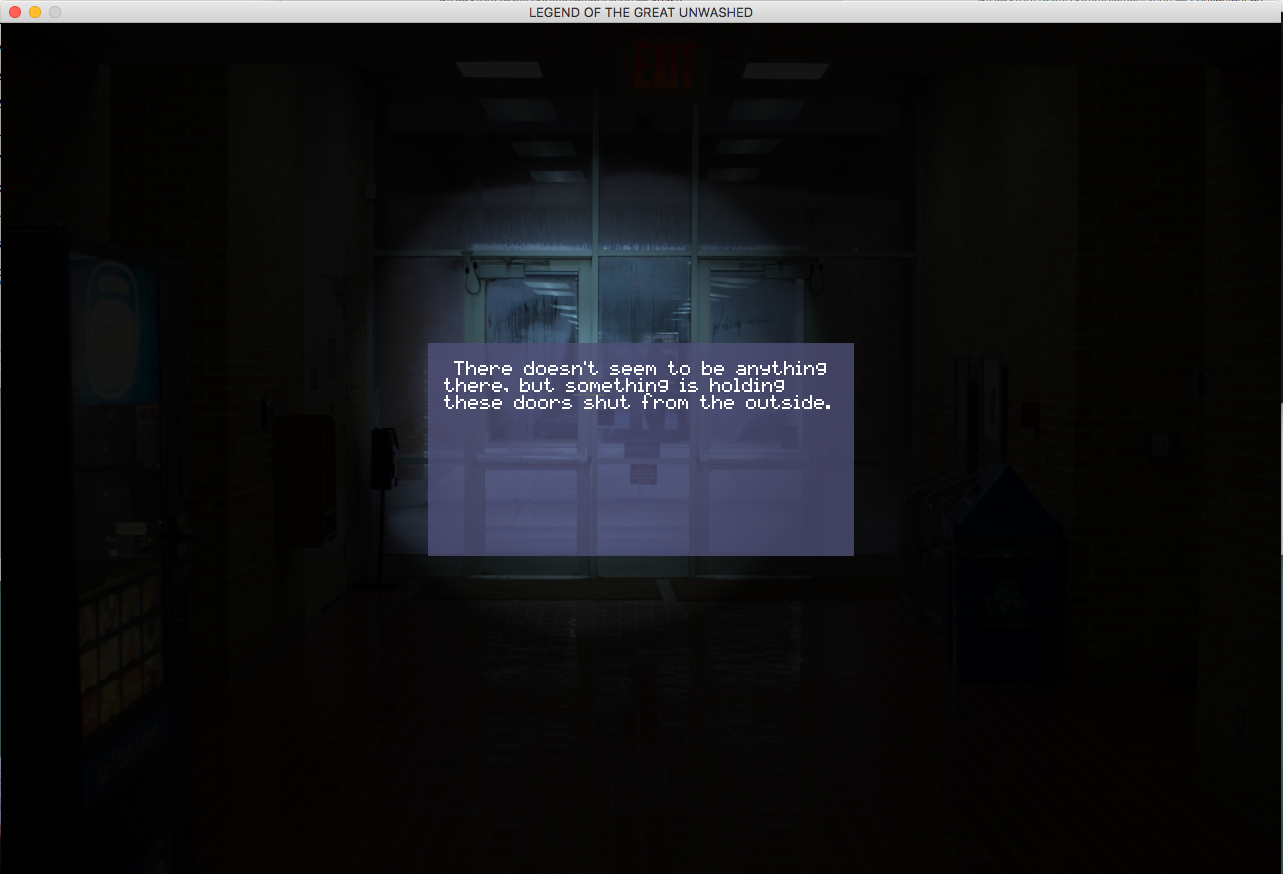
\includegraphics[scale=0.3]{UMimages/textDemo}
		\end{center}
	\subsection{Inventory \& Collectibles}
		The player maintains a collection of items on his or her person, otherwise known as an inventory, and will encounter certain points in the game that require a certain item to proceed. Attempting to pass these areas without that item will cause the game to output a text box informing the player of the required item:\footnote{There is one particular item for which the player will not receive an ``Item required'' text box. This is because that item is integral to the puzzle for an entire level. As such, no hint is provided.}
		\begin{center}
			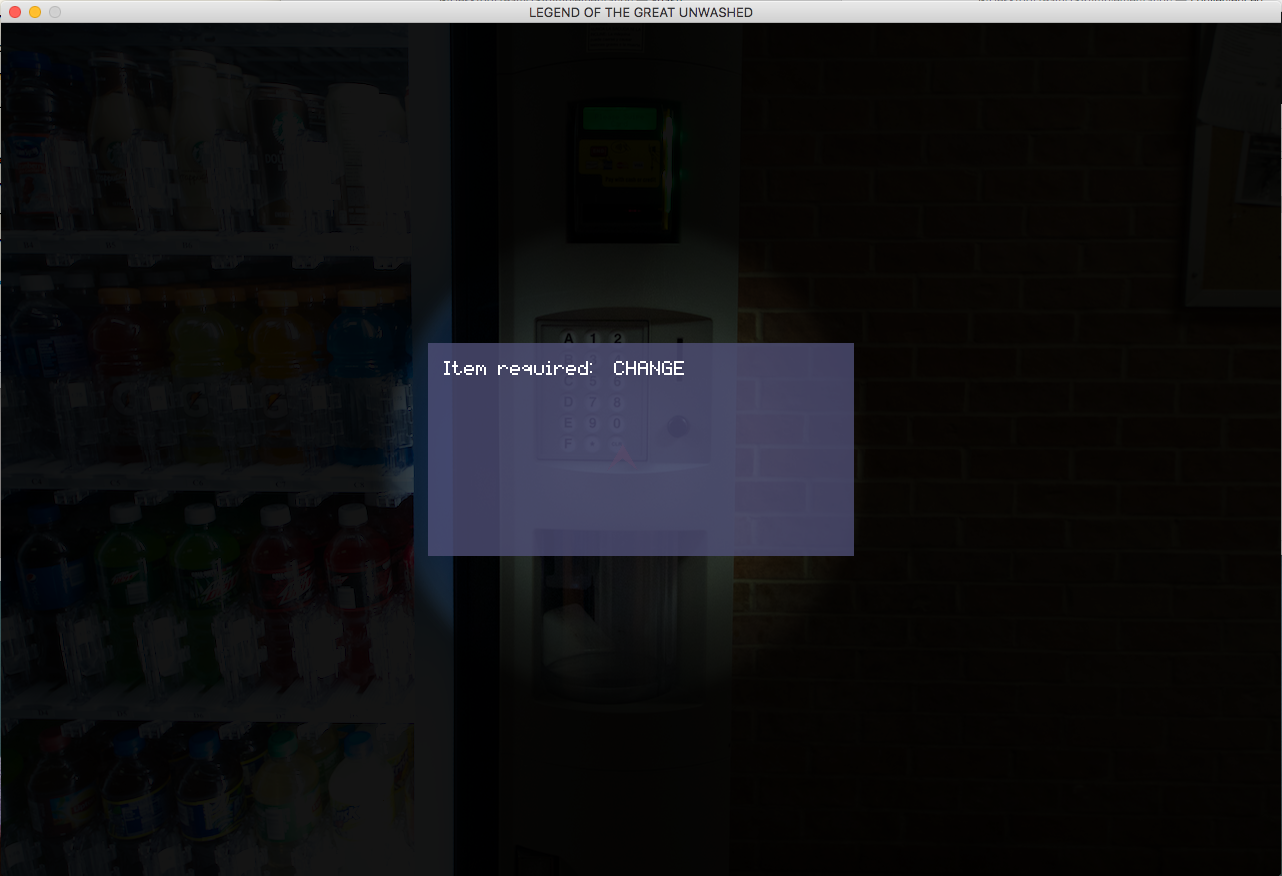
\includegraphics[scale=0.3]{UMimages/invenDemo}
		\end{center}
	\subsection{Death}
		While the player cannot die in the normal sense, there are certain areas in the game where a wrong decision can result in the player's untimely removal from the building and relocation to a more appropriate classroom environment. From this point, the player must trek through the ``purgatory'' area as punishment for their failure, before being allowed another attempt at the puzzles that await inside AB1.\footnote{Upon a player's death, all of the previously solved puzzles and collected inventory items will retain their completed or collected status. Thus, the player can return to where they left off without having to repeatedly complete the same challenges.} There is no limit on the number of times a player can die and respawn in a single game session. 
	\subsection{Victory}
		If the player manages to overcome the hazards of AB1 and submit their Data Structures lab, they will be treated to a king's victory at a destination of their choosing. 


\end{document}